


The fault injection campaign produced largely expected results. The validity and significance of the results are less apparent. Most interesting is the process that yielded the results.


\section{Fault Injection Method}

The fault injection campaign was intended to begin at a higher abstraction level than LLVM bytecode through injecting errors in the benchmarks' source C code. These initial efforts consisted of injecting errors in common places, such as replacing a "<=" with a "<" in a conditional branch. This was largely misguided, as this amounts to mutation testing, and this does not make sense when it does not have anything to validate against. There were no tests that were failing if the benchmark behaved unexpectedly, and there was still outputs provided by the benchmarks. 

Performing mutation testing in the tests that assert the behavior of \taffo{} would allow discussing the developmental fault tolerance of \taffo{}, but this was hindered by the author's lack of experience with \taffo{} development, and the test cases and assertions not being verbose and descriptive enough for an outsider to easily understand what the code was testing. Taking the test in listing~\ref{listing:taffo_unit_test} as an example, one can see that there is a variable annotated for use with \taffo{},  and other variables that are not annotated. A value is returned, but there are no hints as to what the expected behavior given an input is. The function names don't help with this either, nor does the filename, which is test1.c. This makes performing mutation testing a lot more difficult. Mutation testing is used to verify that the tests actually test the behavior they describe, but when the behavior that is being tested is not described, it is all the more difficult to create mutants that target the test in question.

\section{Fault Injection Bit Flip Campaign}

All faults in this campaign were injected in the data bits, not the instruction bits. This puts the fault injection campaign in the same neighborhood as fuzzing, though only one bit is flipped at a time, and there are no other variations in the inputs to the benchmark.

% This comparison is based on injecting faults within the data that is being operated on, not on opcodes or memory locations. This is to verify the change in behavior that changing the variable type incurs.

The results from the fault injection were mostly expected: The deviations from the original answer for the floating point errors started low, then increased exponentially towards the most significant bits.

In the output file of the original floating point implementation without any additional faults injected, there are maximum 19 significant digits in an individual data entry, 16 of which are behind the decimal point. Depending on what the output is used for, an error above 1.0 could be considered to be quite a large error, or it could be insignificant. Figure~\ref{fig:graph_fixed_vs_float_error} shows a graph of the change in error when injecting an error in increasingly more significant bits in a variable. The graph cut-off is set at 1.0, this is to get a better resolution in the lower end of the fault spectrum. In practice, as can be seen in~\ref{table:injection_results}, the highest deviations are a lot higher. The deviation is the output of the comparison script mentioned in section~\ref{section:bitwise_fault_injection}. The x axis describes which bit is flipped, bit number 0 being the least significant bit.

\begin{figure}[h!]
    \centering
    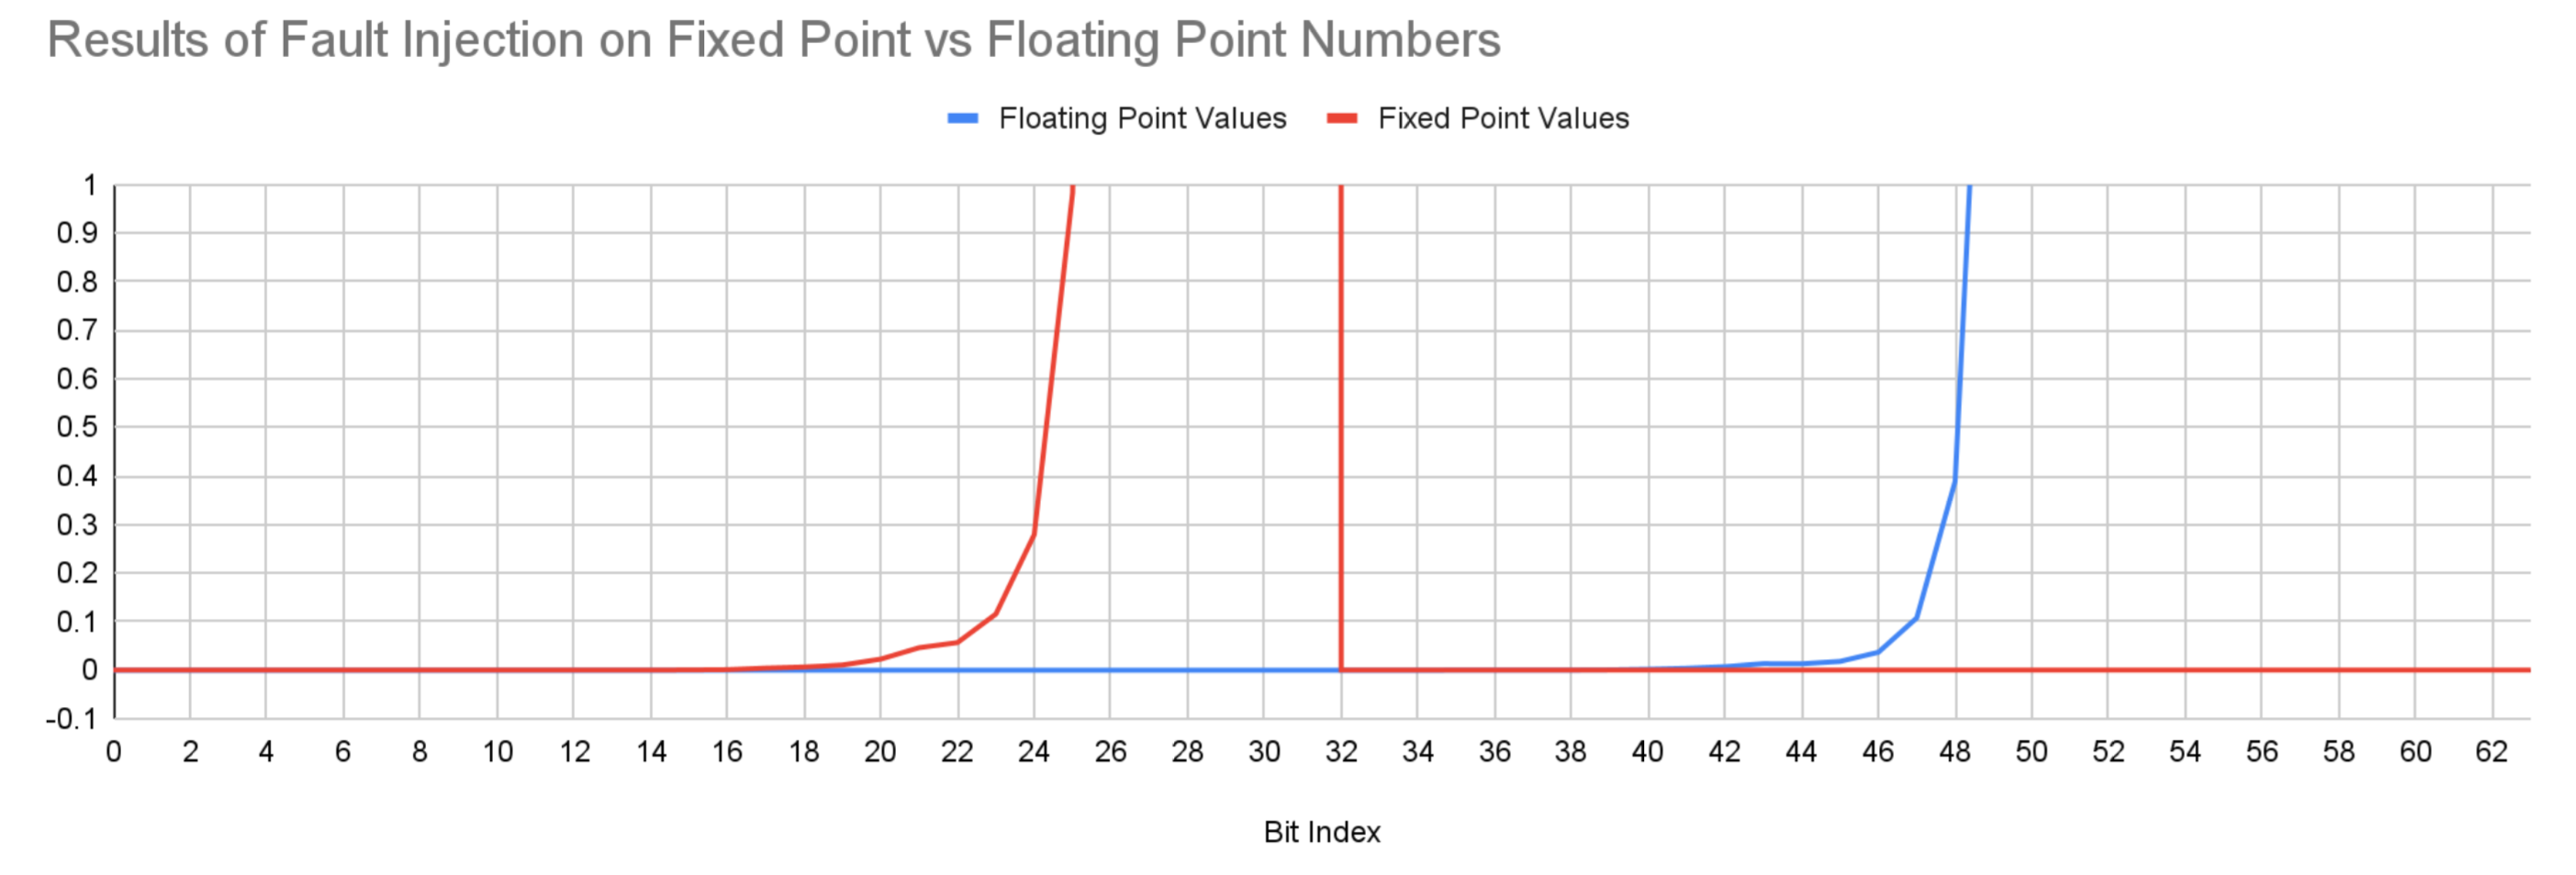
\includegraphics[width=\linewidth]{Images/graph_float_vs_fixed_fault_injection_results.png}
    \caption{The graph shows how the difference from the original floating point version of the program increases the closer to the most significant bit the fault is injected. }
    \label{fig:graph_fixed_vs_float_error}
\end{figure}


The graph y axis starts at negative values even though this is not possible (the y axis is average absolute difference, therefore values will only be positive).This is to more clearly show the line for the floating and fixed point data when the error is small toward the least significant bits.

The graph shows that both the floating point values and the fixed point values initially seem to differ very little from the original non-fault-injected outputs. The difference in the fixed point implementation rises quickly as the injected bit becomes more significant, until suddenly dropping after injection in the bit at index 32. The vertical line that seems to come out of nothing is a part of the continuous fixed point value graph, this is shown clearly in Figure~\ref{fig:zoomed_out_graph}.
\begin{figure}
    \centering
    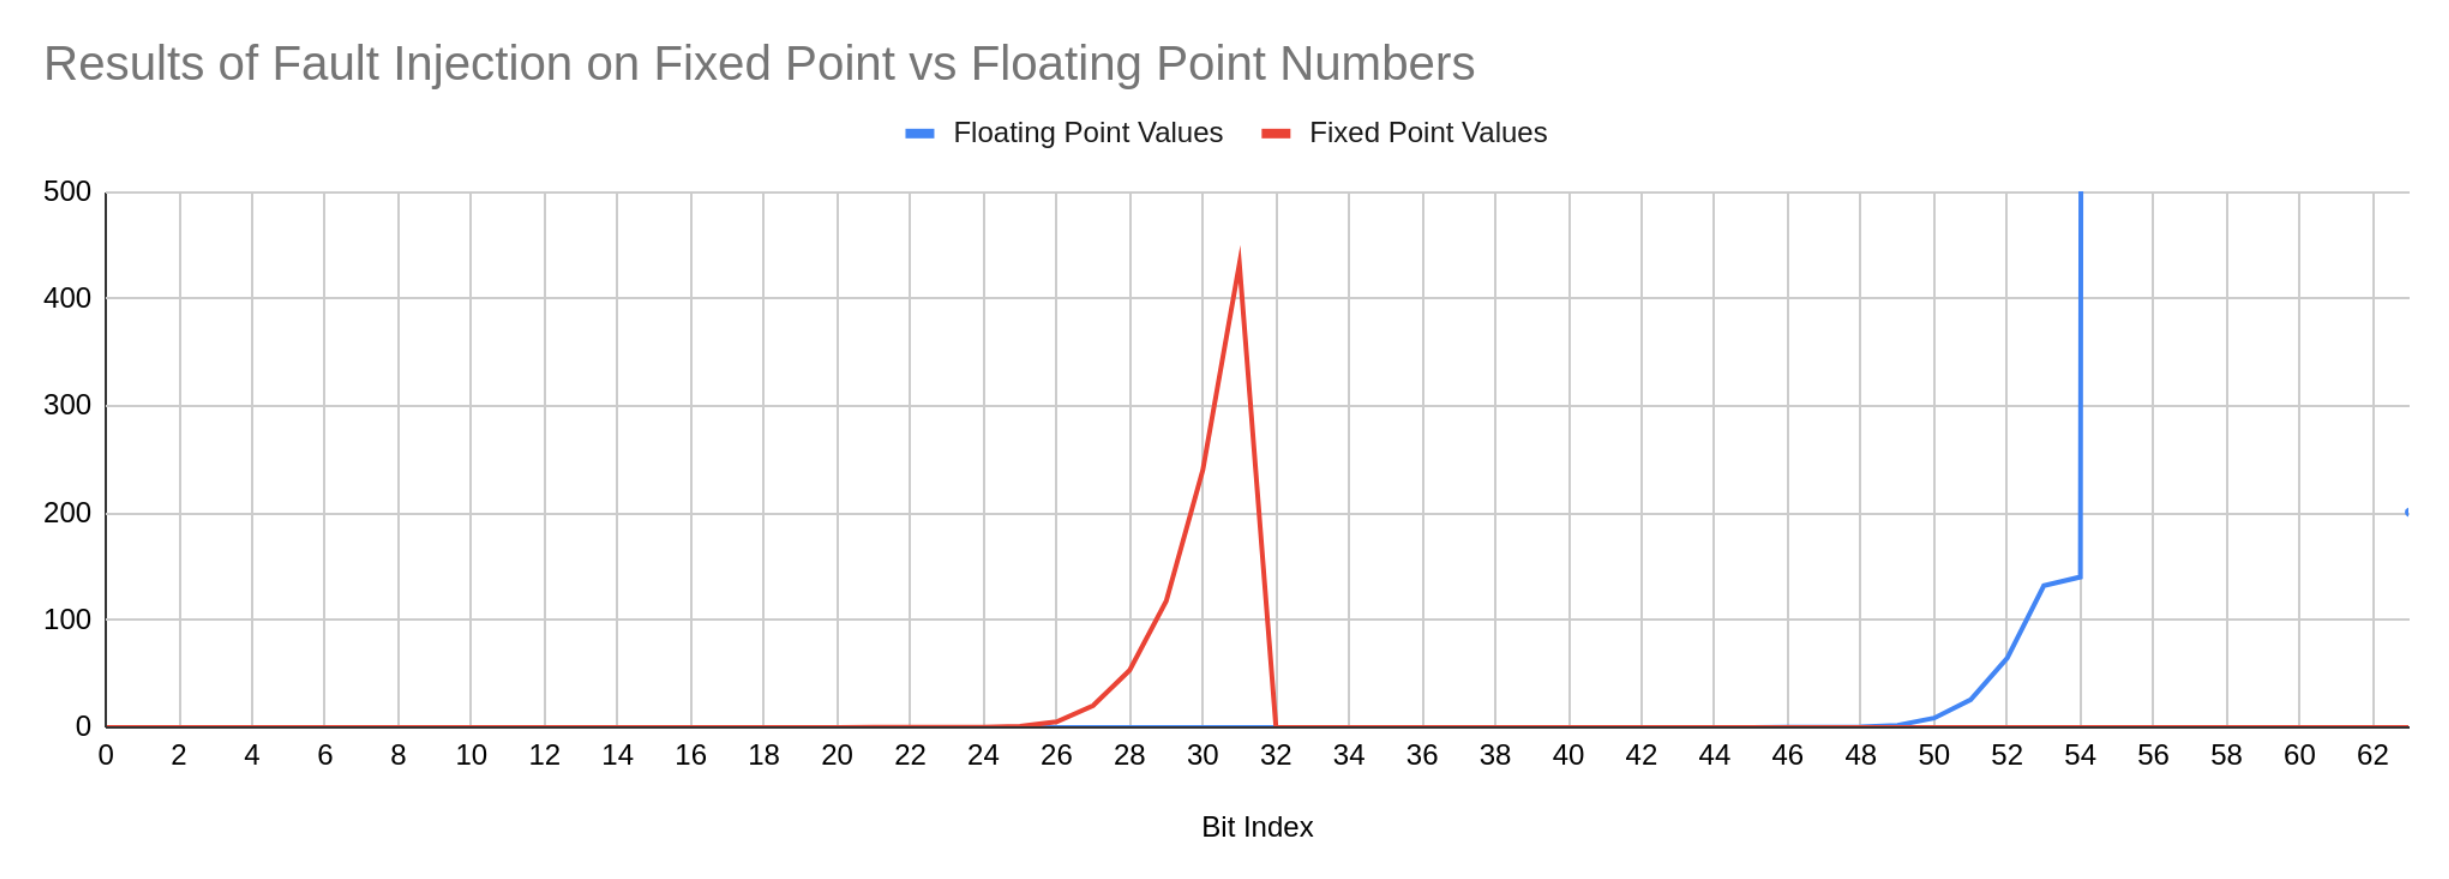
\includegraphics[width=0.75\linewidth]{Images/zoomed_out_graph.png}
    \caption{A zoomed out view of the graph shown in figure~\ref{fig:graph_fixed_vs_float_error} to show all fixed point values.}
    \label{fig:zoomed_out_graph}
\end{figure}

This drop can be explained by looking at the LLVM bytecode that is used to inject the faults, see listing~\ref{listing:llvm_ir_fixed}. Here you can see that while the result of the division is 64 bits, from dividing two 64 bit variables, one of the operands is originally a 32 bit integer that is extended to a 64 bit number. In the final line in the listing, the result of the division and bit flip is then truncated back to a 32 bit integer, thereby discarding the injected bit if it is injected over the bit at index 31, explaining the drop in error after bit 31.

\begin{figure}[h!]
    \centering
    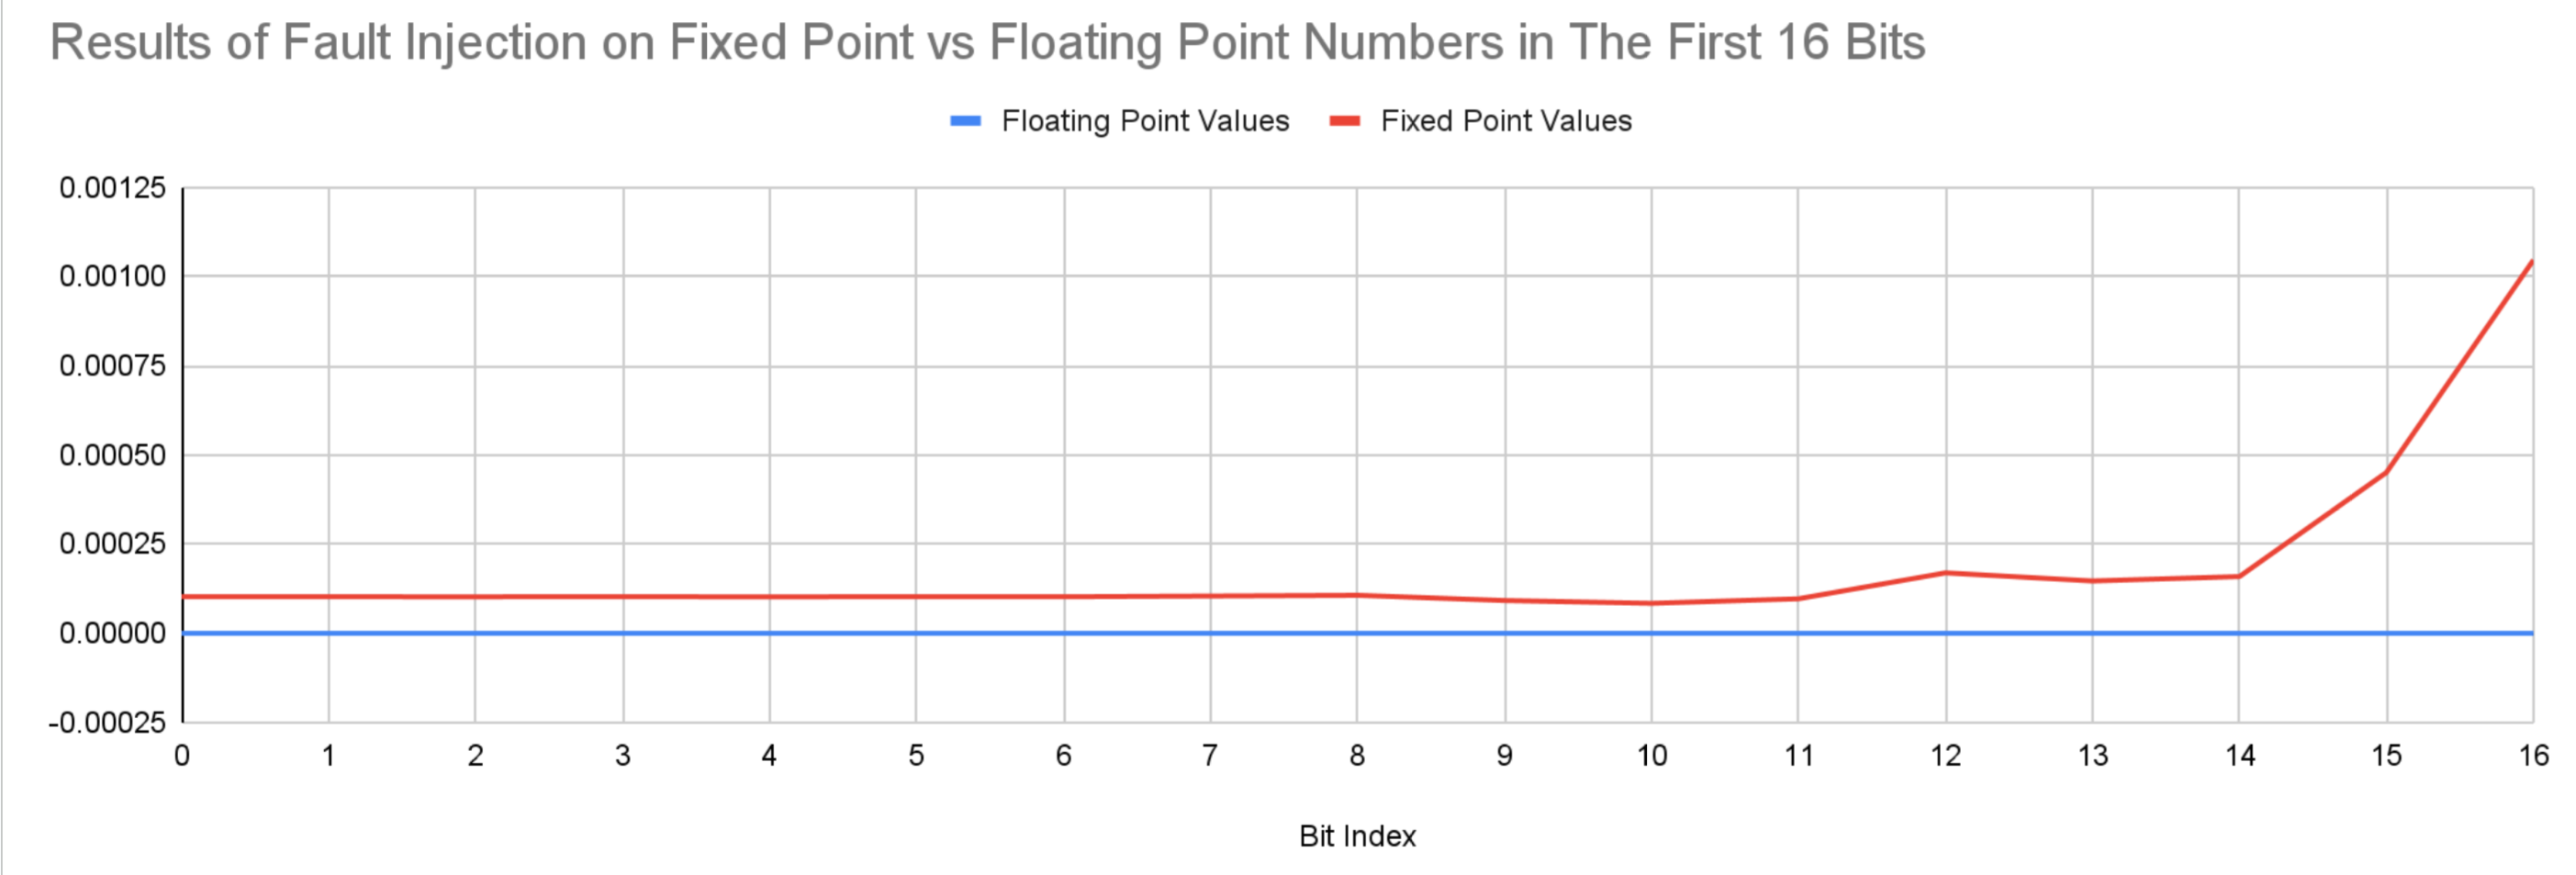
\includegraphics[width=\linewidth]{graph_fault_injection_fix_vs_float_first_16_bits.png}
    \caption{The fixed point error is magnitudes larger than the floating point error at its lowest.}
    \label{fig:graph_fixed_vs_float_error_first_16}
\end{figure}


The fault injection location was selected based on math operations that are only done a few of in the program, such as division, to be able to inject a fault in an equivalent location for both floating point and fixed point versions of the program. The fault injection has only been performed on one benchmark with a limited number of operations, therefore the results may be different in another benchmark stressing another part of the processor. This is partly due to the fact that fixed point and floating point representations require different CPU instructions for mathematical operations. This leads to different code that uses different parts of the processor. 

Some entries and values in the results seem to represent unexpected behavior, but can be explained. The difference for injected bit at index 63 in the floating point version is very low relative to the preceding results, this is due to the most significant bit in the floating point number being the sign bit (resulting in just negating the data input). 
The difference in the fixed point implementation drops significantly after bit index 31. This is because the fixed point number is originally a 32-bit number that is extended to a 64 bit number for the division operation. It gets truncated back to a 32 bit number after the division, discarding changes in the most significant 32 bits of the 64 bit result of the division, therefore not changing the number when injecting a fault in the most significant 32 bits. 

The results of the fault injection campaign completed for the seidel-2d benchmark from the polybench cpu benchmark suite adapted for \taffo{} is not representative for programs compiled with \taffo{} as a whole. The changes that are made to the low-level code vary from project to project depending on the domain, and depends on what the user of the program specifies to be the range of values. 


When assessing how the injected faults affect the program behavior, it is helpful to use the failure classifications found by~\citet{failure_class_with_respect_to_detection} for subtle incorrect and coarse incorrect service values. A service is the behavior of a system as percieved by an external observer. For a perfect observer, i.e. an observer that can accurately map a service output as either a correct or incorrect output. Humans are rarely perfect, which puts us in a different category of observers able to discern between three different states of service delivery: correct, coarse incorrect, and subtle incorrect.  Coarse incorrect are states that are certainly false, correct states are observably correct, and subtle incorrect states are difficult to discern as being incorrect or correct, though they are in reality the result of incorrect service. This means that a value could be percieved as correct while actually being the result of faulty service. This can counterintuitively be a bigger issue than a very large error, in that it can be more difficult to detect~\citep{hodge2004survey}.

This is why the domain matters when discussing reliability. In the result, until injecting a fault in the bit at index 37, the floating point error remains lower than that of the fixed point implementation with no faults injected. In the bit at index 55, the error becomes larger than the highest error recorded for the fixed point implementations, and the error keeps rising until injecting an error at the bit in index 63, which is the sign bit.

If we define the standard fixed point version error as the threshold for a coarse error, the majority of floating point variable bit flips do not constitute a fault. 

For this benchmark, the precision was set so as to allow the use of 32 bit integers for the fixed point implementation. Setting the precision is done through the annotations in the benchmark, and has to be set manually by the programmer.  This was done by the authors of \taffo{} through the use of annotations specifying the range of values that the variables can contain. This may not be the case for all the benchmarks in the included polybench benchmark suite.

% discuss the error, how error rate changes with injected bit, implications taking subtle and coarse errors into account. Subtle errors may have a larger effect on scientific calculations or highly sensitive calculations such as for satellite navigation or space travel, where if travelling very long distances a small error may result in a huge deviation. Larger errors may be easier to discover.
 The fact that many bits in a 64-bit floating point number can be injected without a significant effect on the calculation may be an advantage if the calculation in question is fault tolerant at heart. Floating point errors go up very quickly when the error hits the exponent part of the number, this can be helpful when trying to detect errors from bit flips in floating point numbers. A larger deviation may be easier to discover than a lower deviation, either through statistics or detection algorithms~\citep{hodge2004survey}.


\section{Weaknesses in the Fault Injection Campaign}

The design of the fault injection campaign was influenced by the available approximate computing tools (\taffo\ and Floatsmith). Both tools work using the same principle, reducing precision for compatible computations, so assessing how injecting bits of different significance in reference data affect different internal bit representations/bit widths of numbers is of great interest for both tools. For a tool that does not perform any additional casting operations, this would have been less interesting, though not irrelevant. 

Designing a software fault injection campaign should involve reasoning about the code base: The faults injected should reflect faults that may occur in production environments. This is important for both developmental faults and operational faults because biases in the injection of faults will lead to bias in the results of the fault injection. For instance, injecting developmental faults mainly in  well-tested sections of code may be less relevant than injecting developmental faults in parts of the code that have a lower degree of test coverage if the kind of fault that is injected is caught by the regression tests. 

This fault injection campaign only considers faults of one kind, namely bit flips in supplied data to the kernel. The bit flips are quite drastic as they are injected into every single variable supplied as data to the function. This does not necessarily realistically represent the faults that would occur in production, and gives a more extreme picture of the effect of fault injection on a program that approximates through converting variables to fixed point types. 

Given more time, implementing an approach as outlined by \citet{van2016finding} would be preferable. \citet{van2016finding} maintain that a fault injection campaign requires a good fault model, i.e. an overview of the faults that may occur and in what frequency they occur, and to perform fault injections that follows this fault model. When a fault model does not correspond with the faults that are actually executed during the fault injection campaign, either the fault model is lacking or the fault injection campaign has not gathered enough data. 

According to \citet{van2016finding}, coverage has a significant impact on the fault injection results. Coverage here means the amount of code that is executed throughout the fault injection campaign. If an injected fault is not run throughout the campaign (the fault is not "activated"), the results of the fault injection will not represent the effect of this fault. In this campaign, all the faults injected above the bit in index 31 for the fixed point implementation falls in this category: The fault is truncated away, and is therefore not activated. 

All in all, the focus of the fault injection campaign ended up being on the benchmarks and the tools themselves, not on approximate computing, leading to results that say more about how the benchmark code behaves than the fault injection technique itself. This was due to time constraints caused by focusing too much on using tools that were supposed to simplify fault injection through quickly creating approximate versions of precise programs. Instead of spending time making the tools work, time would have been better spent using approximate computing techniques to manually create multiple versions of the same code, preferably within a domain that allows for clear definitions of both silent data corruptions and hard failures, such as a facial recognition application. The different versions of this approximate computing code would then have their own fault model that reflects the different quirks of the different techniques. 

There are papers that describe approximate computing tools that use a different approach to approximate computing. Of these, Sculptor~\citep{li2018sculptor} and Green~\citep{baek2010green} were promising. Sculptor is described as a tool that implements dynamic loop perforation that is more complex than just removing certain iterations in a loop. Green is a framework that aids a programmer in balancing the need for approximating functions and loops and quality of service, but doesn't itself perform any transformations in code. 

While both papers describe a software tool, the tool is nowhere to be found on the internet. Contacting the authors yielded nothing. 
Reproducibility is one of the most important parts of a scientific report.
It allows researchers to verify the findings independent of the original authors and their biases.
If there is a paper that builds results or data produced by using a program that is either not released or not able to run, the results contained within are not easily verifiable and reproducible. Science that is not verifiable is not very valuable.

\section{Code quality}

% The comparison script written for the fault injection comparison is not perfect either. However, the assumptions are documented, and tests support and explain functionality. 
%This is difficult to realize when using python as a scripting language, but at the very least variable names need to be descriptive, and file outputs need to follow the existing standards and descriptions (for instance not mislabeling an output as a .csv file).

Some faults were apparent not because of the programming skills of the author, but simply because of an IDE tool highlighting errors that were easy to remedy. Figure~\ref{fig:IDE_highlighting} shows the highlighted error, which in this case is a keyword that does nothing. In this case the error is that the code describes functionality that is not possible.

\begin{figure}[h]
    \centering
    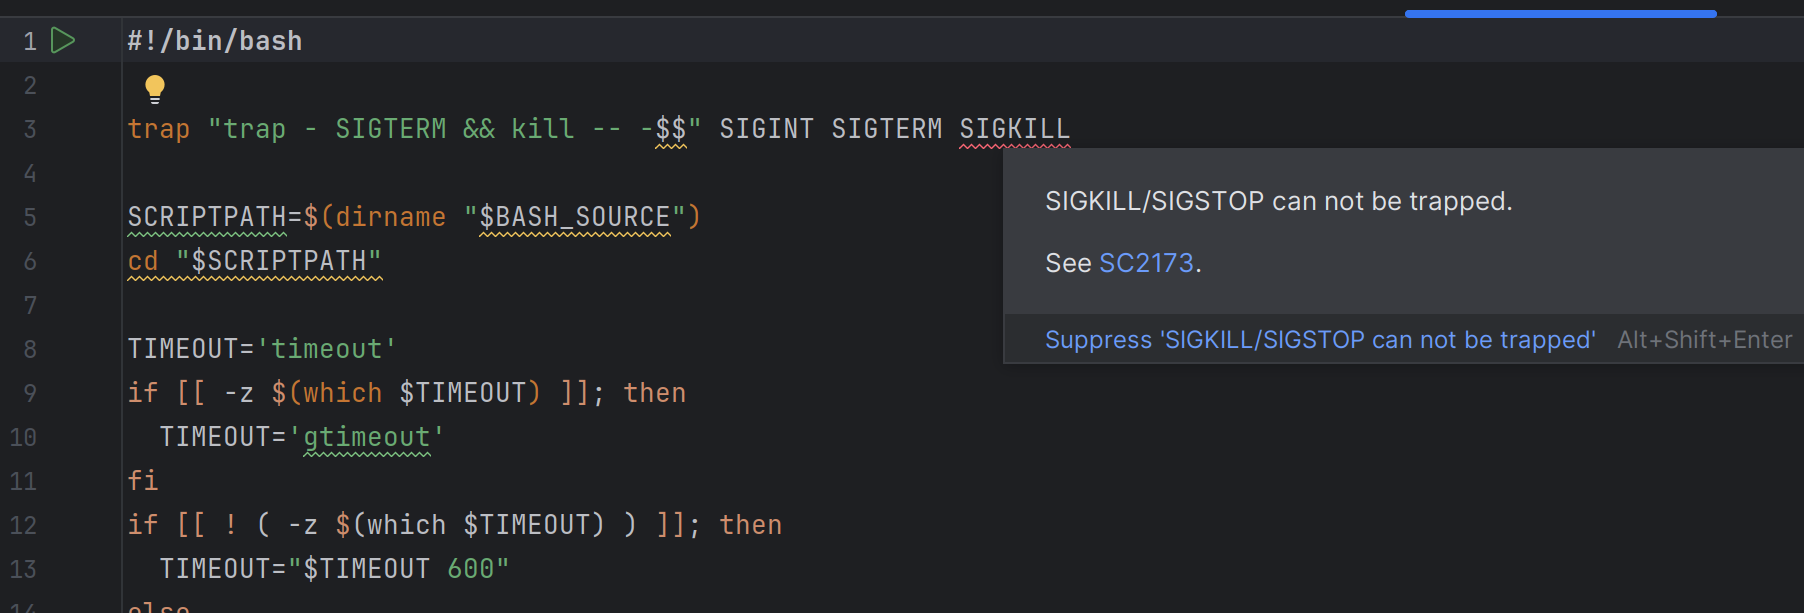
\includegraphics[width=\linewidth]{Images/IDE_highlighting.png}
    \caption{the IDE, in this case CLion, highlighting an error in a shell script.}
    \label{fig:IDE_highlighting}
\end{figure}
% There is a habit of writing code as if to be archived forever. The documentation lags behind, and there is no test suite for the tool

This fault does nothing to affect how the program runs, however it may lead to confusion as it describes behavior that does not actually happen. 


There are many aspects of programming that can be measured to provide an indication of code quality. One such example is test coverage, which measures how many lines of the written code is executed through tests, and a higher percentage of code executed in tests is better. Although a program has 100\% code coverage, this alone does not designate the program as a good program: The tests themselves need to specify what behavior they test, and the test needs to assert that the output aligns with the expected output, such that if there is a change in the code that changes this behavior the test should fail. Quantitative code quality metrics are intended to be used as an aid in writing good code, not as designators of good or bad code. 

Using quantitative code quality metrics is a reliable qualifier of code that is not adequately tested. Taking coverage again as the example metric, while a high coverage cannot be used alone to decide whether code is well written or not, a low coverage is a good indication that the tests do not verify every aspect of the code, or that sections of the code are not being maintained.


\section{Differences between documentation and implementation}

There are discrepancies in \taffo{} which are not documented in neither the code repository nor the papers published about \taffo{}. 
This includes facts such as the error propagator not doing what is described in the papers describing \taffo{},  and the installation instructions of \taffo{} not being foolproof. To enable debugging and further development of \taffo{}, the README specifies that a debug build of LLVM is required. Despite repeated attempts, there has only been one successful install of \taffo{} during the course of this project using a debug build of LLVM, and this successful build was not repeatable despite a clean OS install and following the exact same steps. This included making changes in the source code of a dependency within a \taffo{} dependency.  

The error propagation pass of \taffo{} is by default disabled on the polybench-cpu script that compiles, runs, and evaluates the benchmarks. When enabling it, it produces an estimated maximum error for a specified target in a file given a transformation of the target from floating point to fixed point. This estimation does not correspond to and is in fact quite different from the actual result recorded in the bench-results directory. for instance, for the benchmark 2mm found in the directory linear-algebra/kernel/2mm, the output of the error propagator pass is shown in listing~\ref{listing:error_prop_2mm}.

\begin{lstlisting}[caption=Output of the \taffo{} error propagator for the benchmark 2mm.]
*** Target Errors: ***
Computed error for target D: 3.126388e-14
\end{lstlisting}
\label{listing:error_prop_2mm}

This is quite a lot lower than the actual error recorded when running the fixed point implementation of the benchmark against the floating point implementation, which is 0.1438640358449807895808080808. See the table in appendix~\ref{appendix:vra_2mm} for the complete results for the complete 2mm benchmark results. This difference may be due to a misunderstanding of what the output actually tells us, but this too in itself is part of what has made this project challenging.


Though there is both a test and a test-lit folder in the \taffo{} project neither is documented in the README or elsewhere, and the tests themselves are cryptic. This last fact may be due to the design of LIT itself, which stands for LLVM Integrated Tester. This is the internal framework used within the LLVM project for testing the different compiler tools, and some knowledge of the framework is required to understand the tests. 

In addition to not being very declarative in the test descriptions, the tests folder contains a lot of benchmarks. These are not tests in that they do not assert some kind of functionality that can be verified, only whether the code produces \*some\* output. Therefore it should not reside in the tests folder, but perhaps a folder named benchmarks.

The README file in the simple-test-cases directory in \taffo{} directs a tester to a shell script that builds and runs the test. The makefile marks the directory as tests, which allows for running all the tests in the simple-test-cases directory when building \taffo{} with Cmake.

\begin{lstlisting}[caption=A unit test from the \taffo{} repository]
    ///TAFFO_TEST_ARGS -Xvra -propagate-all


float global;

float test(float param, int notafloat)
{
  int notafloat2;
  float local __attribute((annotate("scalar(range(0, 5.0))")));
  
  local = 2.0;
  local *= param;
  local += notafloat;
  notafloat2 = local;
  return notafloat2;
}

int test2(int a)
{
  return a + 2.0;
}

\end{lstlisting}
\label{listing:taffo_unit_test}

Instead of performing mutation testing on uncertain ground, the initial fault injection was performed directly in LLVM bytecode as described in section~\ref{section:bitwise_fault_injection}.

\taffo{}, when called using the parameters in the existing compile script, produces LLVM bytecode files. These files are numbered according to which optimisation pass they represent in the \taffo{} compilation process. \taffo{} has a flag called emit-llvm that is supposed to emit LLVM bytecode, and does so, but this LLVM bytecode is not linked even though the \taffo{} command specifies that it should be, while also not producing any errors when compiling. To get LLVM bytecode that is linked you need to either link it manually, or take the existing intermediate LLVM bytecode files without specifying the --emit-llvm flag. This was discovered through troubleshooting, and the complete code for extracting the linked, ready-to-fault-inject files can be found in the copied polybench-cpu folder in the cloned \taffo{} repository located at \url{https://github.com/larsj-blip/TAFFO/tree/improve_readability/test/fault-injected-polybench-cpu}, see the file compile\_to\_LLVMIR.sh

